\documentclass{beamer}

\usepackage[utf8]{inputenc}
\usepackage[T1]{fontenc}
\usepackage[english]{babel}
\usepackage[activate={true,nocompatibility},final,kerning=true,spacing=true,factor=1100,stretch=10,shrink=10]{microtype}
\usepackage{amsfonts,amssymb,amsmath}
\usepackage{xcolor}
\usepackage{algorithm}
\usepackage[noend]{algpseudocode}
\usepackage[style=ieee]{biblatex}
\usepackage{booktabs}
\usepackage{hyperref} % load after other packages
\usepackage{todonotes}
\presetkeys{todonotes}{inline}{}
\usepackage[style=ieee]{biblatex}

\usepackage{listings} % code samples with syntax hl
% listings settings
\lstset{ %
  backgroundcolor=\color{white},   % choose the background color; you must add \usepackage{color} or \usepackage{xcolor}; should come as last argument
  basicstyle=\footnotesize,        % the size of the fonts that are used for the code
  breakatwhitespace=false,         % sets if automatic breaks should only happen at whitespace
  breaklines=true,                 % sets automatic line breaking
  captionpos=b,                    % sets the caption-position to bottom
  commentstyle=\color{red},    % comment style
  frame=single,	                   % adds a frame around the code
  keepspaces=true,                 % keeps spaces in text, useful for keeping indentation of code (possibly needs columns=flexible)
  keywordstyle=\color{blue},       % keyword style
  numbers=left,                    % where to put the line-numbers; possible values are (none, left, right)
  numbersep=5pt,                   % how far the line-numbers are from the code
  numberstyle=\tiny\color{gray}, % the style that is used for the line-numbers
  rulecolor=\color{black},         % if not set, the frame-color may be changed on line-breaks within not-black text (e.g. comments (green here))
  stepnumber=2,                    % the step between two line-numbers. If it's 1, each line will be numbered
  stringstyle=\color{mauve},     % string literal style
  tabsize=2,	                   % sets default tabsize to 2 spaces
}




\addbibresource{references.bib}

\makeatletter
\newcommand*{\centerfloat}{%
  \parindent \z@
  \leftskip \z@ \@plus 1fil \@minus \textwidth
  \rightskip\leftskip
  \parfillskip \z@skip}
\makeatother

\DeclareMathOperator*{\argmax}{arg\,max}
\DeclareMathOperator*{\argmin}{arg\,min}

\MakeRobust{\Call}

\renewcommand{\emptyset}{\varnothing}

\newcommand{\ProjectName}{ImputeDB}



\title{\ProjectName{}: A Database for Missing Data}
\author{Jose Cambronero \and Micah Smith \and John K. Feser}
\institute{MIT}
\date{\today{}}

\begin{document}
\frame{\titlepage}

\begin{frame}{Introduction and Motivation}
\begin{itemize}
	\item Handling incorrect or dirty data is a complex and challenging problem for data scientists
	\item $\text{missing data} \subset \text{dirty data}$ and requires imputation/dropping.
	\item Cost of running imputation on entire dataset is a high barrier for analysis.
	\item Lack of flexibility inherent in existing pre-processing approaches.
	\item User should never see missing data or have to modify query. Want a DBMS that 
		allow us to "pretend" data is perfect.
	\item \ProjectName{} allows users to interact with dataset as though it were clean, planning
	around necessary imputation/drops.
\end{itemize}
\end{frame}

\begin{frame}[fragile]{Query Planning: Overview}
\begin{itemize}
	\item $\mu_{min}, \mu_{max}, \delta$: new relational algebra operators
	\item Cost of computation vs. information loss: key tradeoff controlled by $\alpha$ parameter
	\item Placement of operators and dirty sets generated considered in planning.
	\item Histogram transformations used to provide up-to-date cardinality and missing value estimates during planning.
	\item Dynamic programming approach, extends System R optimization\cite{blasgen1981system}
	\item Exponential complexity, but tractable in practice with low planning times.
	\item Imputation operator is a state-of-the-art regression-tree based method.
\end{itemize}
\end{frame}

\begin{frame}[fragile]{Experiments: Queries}
\begin{figure}
  \centerfloat
  \tiny
  \newcounter{queryno}
\begin{tabular}{cl}
\toprule
\# & \multicolumn{1}{c}{Queries on CDC data} \\
\midrule
1 & 
\begin{minipage}{6in}
\begin{lstlisting}[breaklines]
SELECT income, AVG(cuff_size) FROM demo, exams 
WHERE demo.id = exams.id AND height >= 150 GROUP BY income;
\end{lstlisting}
\end{minipage}\refstepcounter{queryno}\label[query]{q1} \\
2 & 
\begin{minipage}{6in}
\begin{lstlisting}[breaklines]
SELECT income, AVG(creatine) FROM demo, exams, labs 
WHERE demo.id = exams.id AND exams.id = labs.id AND income >= 13 AND income <= 15 AND weight >= 63 GROUP BY income;
\end{lstlisting}
\end{minipage}
\refstepcounter{queryno}\label[query]{q2} \\
3 & 
\begin{minipage}{6in}
\begin{lstlisting}[breaklines]
SELECT AVG(blood_lead) FROM demo, exams, labs 
WHERE demo.id = labs.id AND labs.id = exams.id AND age_yrs <= 6;
\end{lstlisting}
\end{minipage}\refstepcounter{queryno}\label[query]{q3}\\
4 & 
\begin{minipage}{6in}
\begin{lstlisting}[breaklines]
SELECT gender, AVG(blood_pressure_systolic) FROM demo, labs, exams 
WHERE demo.id = labs.id AND labs.id = exams.id AND body_mass_index >= 30 GROUP BY gender;
\end{lstlisting}
\end{minipage}\refstepcounter{queryno}\label[query]{q4}\\
5 & 
\begin{minipage}{6in}
\begin{lstlisting}[breaklines]
SELECT AVG(waist_circumference) FROM demo, exams 
WHERE demo.id = exams.id AND height >= 150 AND weight >= 100;
\end{lstlisting}
\end{minipage}\refstepcounter{queryno}\label[query]{q5}\\
  \midrule
\# & \multicolumn{1}{c}{Queries on freeCodeCamp data} \\
\midrule
6 & 
\begin{minipage}{6in}
\begin{lstlisting}[breaklines]
SELECT attendedbootcamp, AVG(income) FROM fcc
WHERE income >= 50000 GROUP BY attendedbootcamp;
\end{lstlisting}
\end{minipage}\refstepcounter{queryno} \label[query]{q6} \\
7 & 
\begin{minipage}{6in}
\begin{lstlisting}[breaklines]
SELECT AVG(commutetime) FROM fcc
WHERE gender = "female" AND countrycitizen = "United States";
\end{lstlisting}
\end{minipage}\refstepcounter{queryno} \label[query]{q7} \\
8 & 
\begin{minipage}{6in}
\begin{lstlisting}[breaklines]
SELECT schooldegree, AVG(studentdebtowe) FROM fcc
WHERE studentdebtowe > 0 GROUP BY schooldegree;
\end{lstlisting}
\end{minipage}\refstepcounter{queryno} \label[query]{q8}\\
9 & 
\begin{minipage}{6in}
\begin{lstlisting}[breaklines]
SELECT attendedbootcamp, AVG(gdp_per_capita) FROM fcc, gdp
WHERE fcc.countrycitizen = gdp.country AND age >= 18
GROUP BY attendedbootcamp;
\end{lstlisting}
\end{minipage}\refstepcounter{queryno} \label[query]{q9}\\
\bottomrule
\end{tabular}

%%% Local Variables:
%%% mode: latex
%%% TeX-master: "main"
%%% End:

  \caption{The queries used in our experiments.}
  \label{fig:queries}
\end{figure}
\end{frame}

\begin{frame}[fragile]{Experiments: Results}
\begin{figure}
  \tiny
  \centerfloat
  \begin{tabular}{cSSSSSSS}
\toprule
\multicolumn{2}{c}{} & \multicolumn{2}{c}{Imputed ($\alpha=0.0$)} & \multicolumn{2}{c}{Imputed ($\alpha=1.0$)} \\
\cmidrule(r){3-4}
\cmidrule(l){5-6}
\# & \multicolumn{1}{c}{Base error} & \multicolumn{1}{c}{Error} & \multicolumn{1}{c}{Time (s)} & \multicolumn{1}{c}{Error} & \multicolumn{1}{c}{Time (s)} \\
\midrule
\ref{q1} & 5.25e+03 & 0.00e+00 & 1.723 & -3.60e+03 & 11.008 \\
\ref{q2} & 3.38e+04 & 0.00e+00 & 1.748 & -3.37e+04 & 10.144 \\
\ref{q3} & 9.32e-04 & 0.00e+00 & 1.732 & 2.54e-02 & 33.04 \\
\ref{q4} & 1.78e+05 & 0.00e+00 & 1.778 & -1.55e+05 & 21.013 \\
\ref{q5} & 9.89e-04 & 0.00e+00 & 1.712 & 9.89e-02 & 7.981 \\
\ref{q6} & 1.01e-02 & 0.00e+00 & 1.982 & 1.13e-02 & 52.309 \\
\ref{q7} & 0.00e+00 & 0.00e+00 & 43M49.786 & 0.00e+00 & 5.946 \\
\ref{q8} & 0.00e+00 & 0.00e+00 & 1.776 & 0.00e+00 & 3.172 \\
\ref{q9} & \multicolumn{1}{c}{--} & \multicolumn{1}{c}{--} & 1.919 & \multicolumn{1}{c}{--} & 2M40.384 \\
\ref{q10} & \multicolumn{1}{c}{--} & \multicolumn{1}{c}{--} & 0.01 & \multicolumn{1}{c}{--} & 7.786 \\
\ref{q11} & \multicolumn{1}{c}{--} & \multicolumn{1}{c}{--} & 0.007 & \multicolumn{1}{c}{--} & 0.103 \\
\ref{q12} & 0.00e+00 & 0.00e+00 & 0.008 & 1.00e-02 & 0.175 \\
\ref{q13} & \multicolumn{1}{c}{--} & \multicolumn{1}{c}{--} & 0.407 & \multicolumn{1}{c}{--} & 0.4 \\
\ref{q14} & 0.00e+00 & 0.00e+00 & 0.752 & 4.37e-01 & 1M14.221 \\
\bottomrule
\end{tabular}

  \caption{Running time and error for queries with different imputation levels.}
  \label{fig:experiments}
\end{figure}
\end{frame}

\begin{frame}
	\center
	Extra slides with details for those interested
\end{frame}

\begin{frame}[fragile]{Motivating Example}
\begin{itemize}
	\item An analyst wants to explore relationships between polling data and survey data on household landline ownership
	\item There is an issue with non-responses in survey data
	\item They issue an ImputeDB query and get an effective response
\end{itemize}

\begin{figure}
\begin{lstlisting}[language=SQL]
SELECT polling.ST, AVG(acs.TEL)
FROM polling, acs
WHERE polling.ST = acs.ST
  AND polling.ERROR > 50         -- 5 percentage points
GROUP BY polling.ST;
\end{lstlisting}
\caption{A typical analyst query on ACS data}
\label{fig:example-query}
\end{figure}
\end{frame}

\begin{frame}[fragile]{Motivating Example: Plan}
\begin{itemize}
	\item ImputeDB adds an impute as necessary for the aggregation
	\item It does not need to impute before then as \verb|acs.ST| is not affected by non-responses and thus has no missing values
\end{itemize}

\begin{figure}[!ht]
    \centering
    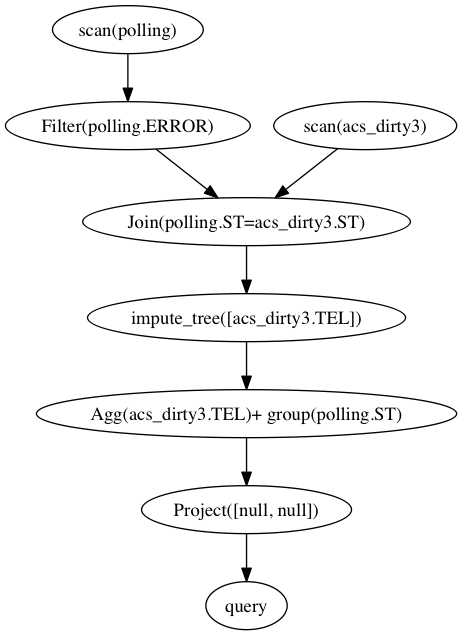
\includegraphics[width=0.4\textwidth]{../paper/figures/example.png}
    \caption{Query plan generated by ImputeDB prioritizing imputation quality.}
    \label{fig:query-plan}
\end{figure}
\end{frame}

\begin{frame}[fragile]{Query Planning: Top-Level Algorithm}

\begin{algorithm}[H]
\scriptsize
\newcommand{\InlineIte}[3]{#2\ \textbf{if}\ #1\ \textbf{else}\ #3}
\renewcommand{\algorithmicindent}{1em}

\begin{algorithmic}[1]
    \Require{
    \Statex
    \begin{itemize}[leftmargin=*,noitemsep]
    \item $q$: A query plan.
    \item $C_l$: A set of attributes that must be imputed in the output of this query plan.
    \item $C_g$: The set of attributes which are used in the final plan.
    \end{itemize}}
  \Function{Impute}{$q,\ C_l,\ C_g$}
  \State $D_{must} \gets \Call{Dirty}{q} \cap C_l$
  \State $D_{may} \gets D_{must} \cup (\Call{Dirty}{q} \cap C_g)$
  \State $Q \gets (\InlineIte{D_{must} = \emptyset}{\{q\}}{\{\mu_{D_{must}}(q),\ \delta_{D_{must}}(q)\}})$
  \State \Return $(\InlineIte{D_{may} = \emptyset}{Q}{Q \cup \{\mu_{D_{may}}(q), \delta_{D_{may}}(q) \}})$
  \EndFunction

  \Statex

  \Require{
    \Statex
    \begin{itemize}[leftmargin=*,noitemsep]
    \item $T$: A set of tables.
    \item $F$: A $T \times \Phi$ relation between tables and filter predicates.
    \item $J$: A $T \times \Psi \times T$ relation between tables and join predicates.
    \item $P$: A set of projection attributes.
    \item $G$: A set of grouping attributes.
    \item $A$: An aggregation function.
    \item $\alpha$: A parameter in $[0, 1]$ that expresses the trade-off between performance and imputation quality.
    \end{itemize}}
  \Function{Plan}{$T,\ F,\ J,\ P,\ G,\ A,\ \alpha$}
  \State $C_g \gets \bigcup_{\psi \in J} \Call{Attr}{\psi}$ \Comment{Collect relevant attributes.}~\label{lst:line:attr-start} 
  \State $C_g \gets C_g\ \cup\ \bigcup_{\phi \in F} \Call{Attr}{\phi}\ \cup\ P \cup\ G\ \cup\ \Call{Attr}{A}$~\label{lst:line:attr-end}
  \Statex
  \State Let $Q$ be an empty plan cache.
  \For{$t \in T$} \Comment{Add selections to the plan cache.}
  \If {$\exists \phi: (t, \phi) \in F$}
  \State $Q[\{t\}] \lhd \{\sigma_{\phi}(q)\ |\ q \in \Call{Impute}{t, \Call{Attrs}{\phi}, C_g}\}$~\label{lst:line:sel}
  \Else\ $Q[\{t\}] \lhd \{t\}$~\label{lst:line:scan}
  \EndIf
  \EndFor
  \Statex
  \For{$size \in 2\dots|T|$} \Comment{Optimize joins.}~\label{lst:line:join}
  \For{$S \in \{\text{all length}\ size\ \text{subsets of}\ T\}$}
  \For{$t \in S$}
  \For{$(t,\ \psi,\ t') \in J$ where $t' \in S \setminus t$}
  \State $L \gets \{\Call{Impute}{q,\ \Call{Attrs}{\psi},\ C_g} ~|~ q \in Q[S \setminus t] \}$
  \State $R \gets \{\Call{Impute}{q,\ \Call{Attrs}{\psi},\ C_g} ~|~ q \in Q[\{t\}] \}$
  \State $Q[S] \lhd \{l \bowtie_\psi r ~|~ l \in L,\ r \in R\}$
  \EndFor
  \EndFor
  \EndFor
  \EndFor
  \Statex
  \State $B \gets Q[T]$ \Comment{Get the best plans for all tables.}
  \If{$G \neq \emptyset$} \Comment{Add optional group \& aggregate.}~\label{lst:line:group}
  \State $C_l \gets G \cup \Call{Attrs}{A}$
  \State $B \gets \bigcup_{q \in B} \{g(q', G, A) ~|~ q' \in \Call{Impute}{q, C_l,\ C_g}\}$
  \EndIf
  
  \State $B \gets \bigcup_{q \in B} \{\pi_P(q') ~|~ q' \in \Call{Impute}{q,\ P,\ P}\}$ \Comment{Add projections.}
  \State \Return $p \in B$ s.t. $p$ is $\alpha$-bound optimal.
  \EndFunction
  
\end{algorithmic}
\caption{A query planner with imputations.}
\label{algo:top-level-planner}

%%% Local Variables:
%%% mode: latex
%%% TeX-master: "../main"
%%% End:

\end{algorithm}

\end{frame}

\begin{frame}[fragile]{Imputation Algorithm}
\begin{itemize}
	\item Iterative algorithm using regression trees: \textit{Chained Equations Regression Trees} (CE-CERT)\cite{burgette2010multiple}
	\item Significant cost to perform on entire dataset
	\item \ProjectName{} allows flexible use
\end{itemize}
\scriptsize

\begin{algorithm}[H]
\scriptsize
  \begin{algorithmic}
    \Require{$T$ is a table. $D$ is a set of attributes of $T$ that need to be imputed, and
      $C$ is a set of attributes of $T$ that have complete data }
    \Ensure{Returns an imputed $T$}
    
    \Function{ImputeWithCE-CART}{$T, D, C$}
    	\State $T' \gets \Call{ImputeRandom}{T, D}$
	\For{$1 ... EPOCHS$}
		\For{$d \in D$}
            \State $imp \gets \Call{TrainRT}{\pi_{C \cup D \backslash \{d\}}(T'), \pi_d{T'}}$
            \State $T' \gets (\pi_{C \cup D \backslash \{d\}}(T'), \Call{PredictRT}{imp, T})$
		\EndFor
	\EndFor
	\Return{$T'$}
	\EndFunction
  \end{algorithmic}
  \caption{An algorithm for chained imputation using regression trees}
  \label{algo:imputation-strategy}

\end{algorithm}
\end{frame}

\begin{frame}[fragile]{Experiments: Data}
\begin{itemize}
	\item Real dataset: American Community Survey (U.S. Census Bureau)
		\begin{itemize}
			\item Preprocessed version courtesy of authors of~\cite{akande2015empirical}.
			\item 671,153 rows and 37 columns, all integers.
			\item Randomly deleted 10\% of fields to create dirtied variant
			\item Can write typical data analyst queries involving filters and aggregates
		\end{itemize}
	\item Synthetic dataset: drawn from uniform distribution $[0,100)$
		\begin{itemize}
			\item10,000 rows and 10 columns
			\item Randomly deleted 30\% ti create dirtied variant
			\item Crafted ad-hoc queries using joins
		\end{itemize}
\end{itemize}
\end{frame}

\begin{frame}[fragile]{Related work}
\begin{itemize}
	\item Long history of imputation in statistical learning community.
		\begin{itemize}
			\item Akande et al (\cite{akande2015empirical}) explored ACS data to compare imputation strategies.
			\item Burgette and Reiter (\cite{burgette2010multiple}) introduce sequences of regression trees.
		\end{itemize}
	\item Long history of null value semantics in database community.
		\begin{itemize}
			\item Treatment of nulls described as early as  \cite{codd1973understanding}
			\item Statistical databases, such as BayesDB (\cite{mansinghka2015bayesdb}) combine statistical inference techniques and traditional querying.
		\end{itemize}
	\item \ProjectName{} first to integrate imputation into query planning with cost-based optimizer.
	\item \ProjectName{} treatment of nulls completely abstracted from user perspective: SQL logical independence.
\end{itemize}
\end{frame}


\begin{frame}[fragile]{Conclusion and Future work}
\begin{itemize}
	\item Missing values and their imputation can successfully be integrated into the relational calculus
	\item By taking a dynamic programming approach, we can consider a variety of operator placements
and input columns, while keeping planning tractable in real-world examples.
	\item Considered series of real-world and fabricated queries, showing viability of approach.
	\item Future work:
		\begin{itemize}
			\item Extend imputation operators with global information (\textit{impute by need})
			\item Introduce multiple imputation algorithms into optimizer for consideration in plans \
			\item Implement in a production-quality database.
		\end{itemize}
\end{itemize}
\end{frame}

\begin{frame}[t,allowframebreaks]{References}
  \nocite{*}
  \printbibliography
 \end{frame}


\end{document}
